% \section{Visualization design}
% \subsection{Query execution overview}
% \subsubsection{Execution plan view}
% \subsubsection{Execution progress view}
% \subsection{Task view}
% \subsection{System profiling visualization}
% \subsection{Linkage and interactions}

\section{Visualization design}
Following the data modeling, we present the web-based visual analytics system to support the interactive exploration with four coordinated views. The Execution progress demonstrates the overview about how the query plan are execute(\textbf{T1}), the Task distribution view shows the task distribution and the data dependencies. Integrated with the machine performance metrics, this view is also used for reason the specific patterns of tasks(\textbf{T2} and \textbf{T3}).  Task list provides the detailed information at the task level(\textbf{T2}).  At last, the interaction and linkage are introduced to support the multi-level explorations(\textbf{T4}).

\subsection{Query Progress View}


\begin{figure}[t]
	\centering
	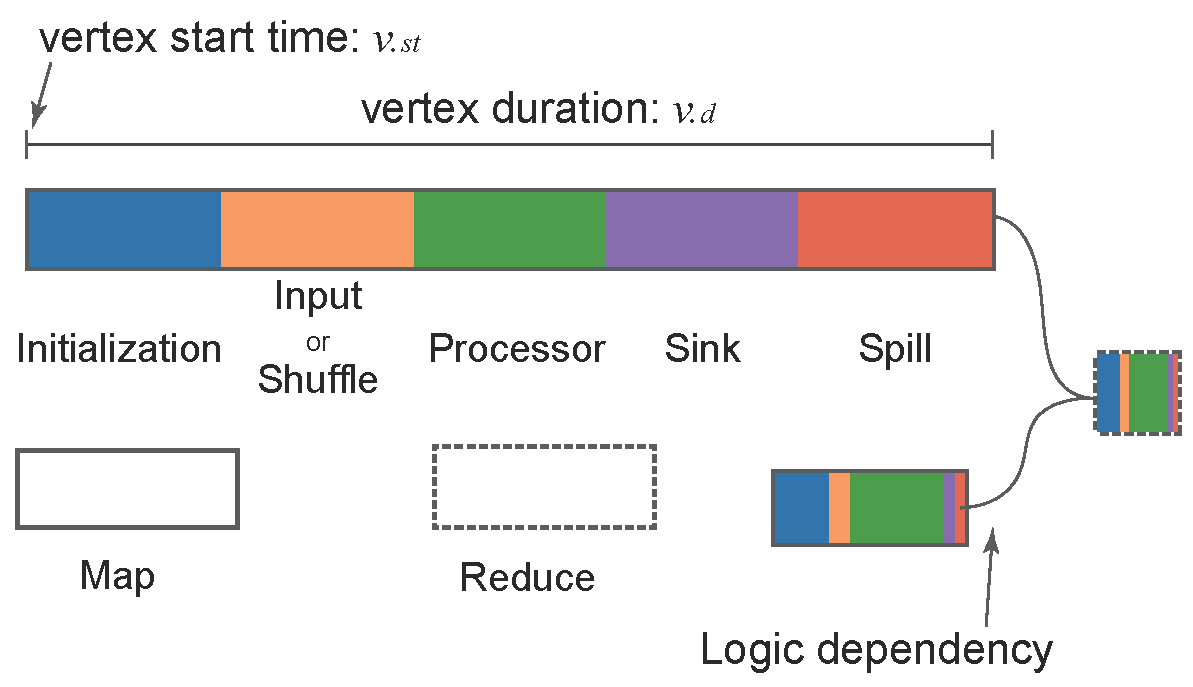
\includegraphics[width=0.40\textwidth]{figures/visualization/progressdesign.pdf}
	\vspace{-3mm}
	\caption{Visual encoding of logic vertex and dependency}
	\label{fig:progress}
	\vspace{-3mm}
\end{figure}


Query Progress View is developed to overview the overall progress of query execution and the logic dependencies. 
The commonly used methods to visualize the progress data is Gantt chart.

As shown by figure~\ref{fig:progress}, the x-axis indicates the timestamp. The rectangles with the same  height indicate the temporal information of logic vertices. Given a vertex $v$, the position of left sides indicates the start time $v.st$ and the duration of $v.d$ is encoded by the length of the rectangle. We use the color to encode the step and the stroke dash style to encode the type of vertex as shown by figure~\ref{fig:progress}.

%\begin{itemize}
%    \item Traditional method: Gantt diagram and design consideration 
%    \item Proposed algorithms, link processing
%    \item Alternative design
%        \begin{itemize}
%            \item Gantt(consider the vertical edge, large space, unclear structure)
%            \item New design loose(clear structure, large space)
%            \item New design compact(small space, unclear structure    )
%        \end{itemize}
%\end{itemize}

% -Visual form of Gantt diagram
% -Our design consideration
% -Algorithms
% -Design alternatives
% --gantt(consider the vertical edge, large space, unclear structure)
% --new design loose(clear structure, large space)
% --new design compact(small space, unclear structure)
% --new design compact, edge processing(small space, clear structure)
\subsection{Pattern Explorer}

Pattern Explorer is developed to provide efficient pattern discovery and reasoning at the task-level. This component consists of multiple coordinated views, including Distribution View and Performance View.
\subsubsection{Distribution View}

The Distribution View is designed to explore the temporal pattern and dependencies of tasks.
Before our collaboration, the domain experts use Gantt Chart Diagram to display the overall progress of tasks, shown in figure~\ref{**}. 
However, Gantt Chart Diagram-based methods suffer significant scalability problem in our applications. Hundreds to thousands of tasks are associated with a vertex in our scenario, which requires a very large space to place all the horizontal bars. 
Moreover, visualizing a large number of bars in this way is difficult for users to compare the absolute length of the tasks due to the lack of alignment~\ref{}, which hinders the users' ability to discover the group-based patterns or identify the abnormal tasks. 

To tackle this issue, we develop a visualization with a square shape of rendering canvas as the basis. As shown in Figure~\ref{**}, the vertical axis(from top to bottom) indicates the start time, and the horizontal axis(from left to right) indicates the end time. This design has two benefits: 1) we simplify each horizontal bar as dots. Thus the tasks can be presented as the point cloud in the canvas. This presentation form may result in the visual clutter caused by the gathering and overlap of points, but can significantly highlight the clusters and outliers, which can help the users to find the task of interest; 2) we linearly map the time range to both horizontal and vertical axis. In this way, the horizontal distance from point to the diagonal line of canvas can be used to represent the duration of the task, which helps the users to compare the task duration. 

According to current 
% \begin{itemize}
%     \item Design consideration. Why gantt doesn't work(need very large space, difficult to show the data-flow link, difficult to show and select the abnormal cases)
%     \item Our design
%     \item Compare with design alternative (Gantt)
% \end{itemize}


\subsection{Profiling view}
\begin{itemize}
    \item Our design consideration
    \item Design: Embedding task view to profiling view
    \item Design: Visualize the profiling results
\end{itemize}

\subsection{Interactions}
\begin{itemize}
    \item Multi-scale navigation
    \item Inner and inter linking
\end{itemize}
